\documentclass[1p]{elsarticle_modified}
%\bibliographystyle{elsarticle-num}

%\usepackage[colorlinks]{hyperref}
%\usepackage{abbrmath_seonhwa} %\Abb, \Ascr, \Acal ,\Abf, \Afrak
\usepackage{amsfonts}
\usepackage{amssymb}
\usepackage{amsmath}
\usepackage{amsthm}
\usepackage{scalefnt}
\usepackage{amsbsy}
\usepackage{kotex}
\usepackage{caption}
\usepackage{subfig}
\usepackage{color}
\usepackage{graphicx}
\usepackage{xcolor} %% white, black, red, green, blue, cyan, magenta, yellow
\usepackage{float}
\usepackage{setspace}
\usepackage{hyperref}

\usepackage{tikz}
\usetikzlibrary{arrows}

\usepackage{multirow}
\usepackage{array} % fixed length table
\usepackage{hhline}

%%%%%%%%%%%%%%%%%%%%%
\makeatletter
\renewcommand*\env@matrix[1][\arraystretch]{%
	\edef\arraystretch{#1}%
	\hskip -\arraycolsep
	\let\@ifnextchar\new@ifnextchar
	\array{*\c@MaxMatrixCols c}}
\makeatother %https://tex.stackexchange.com/questions/14071/how-can-i-increase-the-line-spacing-in-a-matrix
%%%%%%%%%%%%%%%

\usepackage[normalem]{ulem}

\newcommand{\msout}[1]{\ifmmode\text{\sout{\ensuremath{#1}}}\else\sout{#1}\fi}
%SOURCE: \msout is \stkout macro in https://tex.stackexchange.com/questions/20609/strikeout-in-math-mode

\newcommand{\cancel}[1]{
	\ifmmode
	{\color{red}\msout{#1}}
	\else
	{\color{red}\sout{#1}}
	\fi
}

\newcommand{\add}[1]{
	{\color{blue}\uwave{#1}}
}

\newcommand{\replace}[2]{
	\ifmmode
	{\color{red}\msout{#1}}{\color{blue}\uwave{#2}}
	\else
	{\color{red}\sout{#1}}{\color{blue}\uwave{#2}}
	\fi
}

\newcommand{\Sol}{\mathcal{S}} %segment
\newcommand{\D}{D} %diagram
\newcommand{\A}{\mathcal{A}} %arc


%%%%%%%%%%%%%%%%%%%%%%%%%%%%%5 test

\def\sl{\operatorname{\textup{SL}}(2,\Cbb)}
\def\psl{\operatorname{\textup{PSL}}(2,\Cbb)}
\def\quan{\mkern 1mu \triangleright \mkern 1mu}

\theoremstyle{definition}
\newtheorem{thm}{Theorem}[section]
\newtheorem{prop}[thm]{Proposition}
\newtheorem{lem}[thm]{Lemma}
\newtheorem{ques}[thm]{Question}
\newtheorem{cor}[thm]{Corollary}
\newtheorem{defn}[thm]{Definition}
\newtheorem{exam}[thm]{Example}
\newtheorem{rmk}[thm]{Remark}
\newtheorem{alg}[thm]{Algorithm}

\newcommand{\I}{\sqrt{-1}}
\begin{document}

%\begin{frontmatter}
%
%\title{Boundary parabolic representations of knots up to 8 crossings}
%
%%% Group authors per affiliation:
%\author{Yunhi Cho} 
%\address{Department of Mathematics, University of Seoul, Seoul, Korea}
%\ead{yhcho@uos.ac.kr}
%
%
%\author{Seonhwa Kim} %\fnref{s_kim}}
%\address{Center for Geometry and Physics, Institute for Basic Science, Pohang, 37673, Korea}
%\ead{ryeona17@ibs.re.kr}
%
%\author{Hyuk Kim}
%\address{Department of Mathematical Sciences, Seoul National University, Seoul 08826, Korea}
%\ead{hyukkim@snu.ac.kr}
%
%\author{Seokbeom Yoon}
%\address{Department of Mathematical Sciences, Seoul National University, Seoul, 08826,  Korea}
%\ead{sbyoon15@snu.ac.kr}
%
%\begin{abstract}
%We find all boundary parabolic representation of knots up to 8 crossings.
%
%\end{abstract}
%\begin{keyword}
%    \MSC[2010] 57M25 
%\end{keyword}
%
%\end{frontmatter}

%\linenumbers
%\tableofcontents
%
\newcommand\colored[1]{\textcolor{white}{\rule[-0.35ex]{0.8em}{1.4ex}}\kern-0.8em\color{red} #1}%
%\newcommand\colored[1]{\textcolor{white}{ #1}\kern-2.17ex	\textcolor{white}{ #1}\kern-1.81ex	\textcolor{white}{ #1}\kern-2.15ex\color{red}#1	}

{\Large $\underline{12n_{0459}~(K12n_{0459})}$}

\setlength{\tabcolsep}{10pt}
\renewcommand{\arraystretch}{1.6}
\vspace{1cm}\begin{tabular}{m{100pt}>{\centering\arraybackslash}m{274pt}}
\multirow{5}{120pt}{
	\centering
	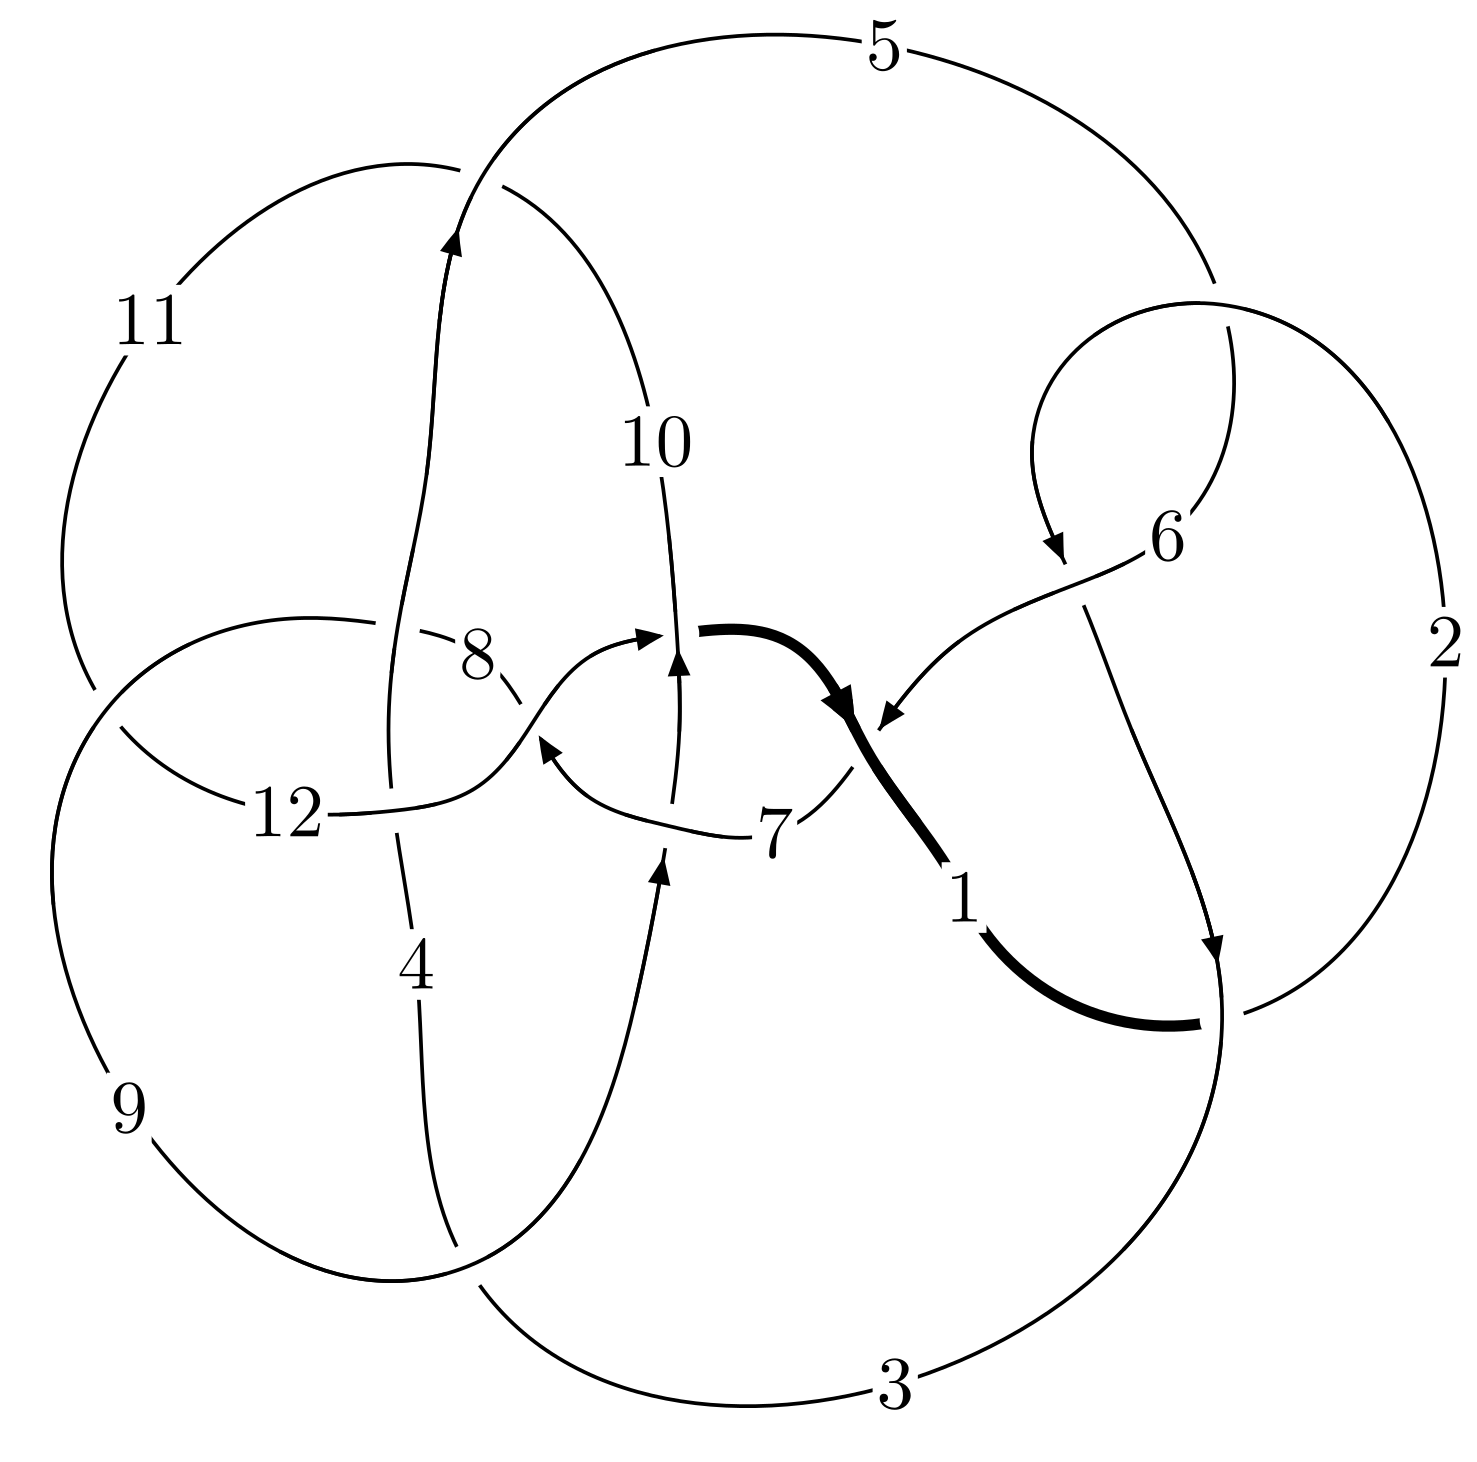
\includegraphics[width=112pt]{../../../GIT/diagram.site/Diagrams/png/2548_12n_0459.png}\\
\ \ \ A knot diagram\footnotemark}&
\allowdisplaybreaks
\textbf{Linearized knot diagam} \\
\cline{2-2}
 &
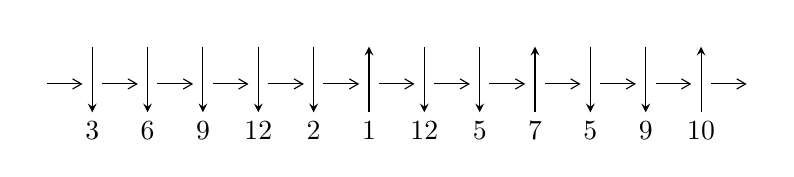
\begin{tikzpicture}[x=20pt, y=17pt]
	% nodes
	\node (C0) at (0, 0) {};
	\node (C1) at (1, 0) {};
	\node (C1U) at (1, +1) {};
	\node (C1D) at (1, -1) {3};

	\node (C2) at (2, 0) {};
	\node (C2U) at (2, +1) {};
	\node (C2D) at (2, -1) {6};

	\node (C3) at (3, 0) {};
	\node (C3U) at (3, +1) {};
	\node (C3D) at (3, -1) {9};

	\node (C4) at (4, 0) {};
	\node (C4U) at (4, +1) {};
	\node (C4D) at (4, -1) {12};

	\node (C5) at (5, 0) {};
	\node (C5U) at (5, +1) {};
	\node (C5D) at (5, -1) {2};

	\node (C6) at (6, 0) {};
	\node (C6U) at (6, +1) {};
	\node (C6D) at (6, -1) {1};

	\node (C7) at (7, 0) {};
	\node (C7U) at (7, +1) {};
	\node (C7D) at (7, -1) {12};

	\node (C8) at (8, 0) {};
	\node (C8U) at (8, +1) {};
	\node (C8D) at (8, -1) {5};

	\node (C9) at (9, 0) {};
	\node (C9U) at (9, +1) {};
	\node (C9D) at (9, -1) {7};

	\node (C10) at (10, 0) {};
	\node (C10U) at (10, +1) {};
	\node (C10D) at (10, -1) {5};

	\node (C11) at (11, 0) {};
	\node (C11U) at (11, +1) {};
	\node (C11D) at (11, -1) {9};

	\node (C12) at (12, 0) {};
	\node (C12U) at (12, +1) {};
	\node (C12D) at (12, -1) {10};
	\node (C13) at (13, 0) {};

	% arrows
	\draw[->,>={angle 60}]
	(C0) edge (C1) (C1) edge (C2) (C2) edge (C3) (C3) edge (C4) (C4) edge (C5) (C5) edge (C6) (C6) edge (C7) (C7) edge (C8) (C8) edge (C9) (C9) edge (C10) (C10) edge (C11) (C11) edge (C12) (C12) edge (C13) ;	\draw[->,>=stealth]
	(C1U) edge (C1D) (C2U) edge (C2D) (C3U) edge (C3D) (C4U) edge (C4D) (C5U) edge (C5D) (C6D) edge (C6U) (C7U) edge (C7D) (C8U) edge (C8D) (C9D) edge (C9U) (C10U) edge (C10D) (C11U) edge (C11D) (C12D) edge (C12U) ;
	\end{tikzpicture} \\
\hhline{~~} \\& 
\textbf{Solving Sequence} \\ \cline{2-2} 
 &
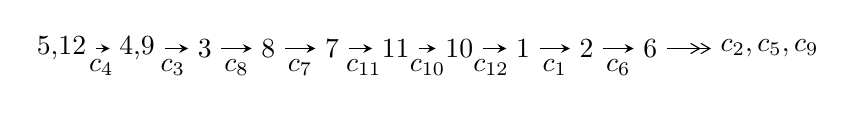
\begin{tikzpicture}[x=23pt, y=7pt]
	% node
	\node (A0) at (-1/8, 0) {5,12};
	\node (A1) at (17/16, 0) {4,9};
	\node (A2) at (17/8, 0) {3};
	\node (A3) at (25/8, 0) {8};
	\node (A4) at (33/8, 0) {7};
	\node (A5) at (41/8, 0) {11};
	\node (A6) at (49/8, 0) {10};
	\node (A7) at (57/8, 0) {1};
	\node (A8) at (65/8, 0) {2};
	\node (A9) at (73/8, 0) {6};
	\node (C1) at (1/2, -1) {$c_{4}$};
	\node (C2) at (13/8, -1) {$c_{3}$};
	\node (C3) at (21/8, -1) {$c_{8}$};
	\node (C4) at (29/8, -1) {$c_{7}$};
	\node (C5) at (37/8, -1) {$c_{11}$};
	\node (C6) at (45/8, -1) {$c_{10}$};
	\node (C7) at (53/8, -1) {$c_{12}$};
	\node (C8) at (61/8, -1) {$c_{1}$};
	\node (C9) at (69/8, -1) {$c_{6}$};
	\node (A10) at (11, 0) {$c_{2},c_{5},c_{9}$};

	% edge
	\draw[->,>=stealth]	
	(A0) edge (A1) (A1) edge (A2) (A2) edge (A3) (A3) edge (A4) (A4) edge (A5) (A5) edge (A6) (A6) edge (A7) (A7) edge (A8) (A8) edge (A9) ;
	\draw[->>,>={angle 60}]	
	(A9) edge (A10);
\end{tikzpicture} \\ 

\end{tabular} \\

\footnotetext{
The image of knot diagram is generated by the software ``\textbf{Draw programme}" developed by Andrew Bartholomew(\url{http://www.layer8.co.uk/maths/draw/index.htm\#Running-draw}), where we modified some parts for our purpose(\url{https://github.com/CATsTAILs/LinksPainter}).
}\phantom \\ \newline 
\centering \textbf{Ideals for irreducible components\footnotemark of $X_{\text{par}}$} 
 
\begin{align*}
I^u_{1}&=\langle 
b- u,\;-2.55290\times10^{42} u^{36}+5.44795\times10^{42} u^{35}+\cdots+1.76508\times10^{43} a-3.00825\times10^{43},\\
\phantom{I^u_{1}}&\phantom{= \langle  }u^{37}- u^{36}+\cdots+3 u-1\rangle \\
I^u_{2}&=\langle 
b+u,\;250 u^{18}-299 u^{17}+\cdots+73 a+547,\;u^{19}- u^{18}+\cdots+3 u+1\rangle \\
I^u_{3}&=\langle 
2.39883\times10^{77} u^{33}+4.38682\times10^{77} u^{32}+\cdots+2.11269\times10^{80} b+4.67078\times10^{80},\\
\phantom{I^u_{3}}&\phantom{= \langle  }-2.66819\times10^{80} u^{33}-6.63024\times10^{80} u^{32}+\cdots+4.21058\times10^{83} a-5.18491\times10^{83},\\
\phantom{I^u_{3}}&\phantom{= \langle  }u^{34}+u^{33}+\cdots+1952 u-1993\rangle \\
\\
\end{align*}
\raggedright * 3 irreducible components of $\dim_{\mathbb{C}}=0$, with total 90 representations.\\
\footnotetext{All coefficients of polynomials are rational numbers. But the coefficients are sometimes approximated in decimal forms when there is not enough margin.}
\newpage
\renewcommand{\arraystretch}{1}
\centering \section*{I. $I^u_{1}= \langle b- u,\;-2.55\times10^{42} u^{36}+5.45\times10^{42} u^{35}+\cdots+1.77\times10^{43} a-3.01\times10^{43},\;u^{37}- u^{36}+\cdots+3 u-1 \rangle$}
\flushleft \textbf{(i) Arc colorings}\\
\begin{tabular}{m{7pt} m{180pt} m{7pt} m{180pt} }
\flushright $a_{5}=$&$\begin{pmatrix}1\\0\end{pmatrix}$ \\
\flushright $a_{12}=$&$\begin{pmatrix}0\\u\end{pmatrix}$ \\
\flushright $a_{4}=$&$\begin{pmatrix}1\\- u^2\end{pmatrix}$ \\
\flushright $a_{9}=$&$\begin{pmatrix}0.144634 u^{36}-0.308653 u^{35}+\cdots-1.70408 u+1.70432\\u\end{pmatrix}$ \\
\flushright $a_{3}=$&$\begin{pmatrix}0.0641583 u^{36}-0.204773 u^{35}+\cdots-2.93838 u+1.14286\\0.00595874 u^{36}-0.0145660 u^{35}+\cdots+0.258814 u-0.0315982\end{pmatrix}$ \\
\flushright $a_{8}=$&$\begin{pmatrix}0.144634 u^{36}-0.308653 u^{35}+\cdots-0.704084 u+1.70432\\u\end{pmatrix}$ \\
\flushright $a_{7}=$&$\begin{pmatrix}0.144634 u^{36}-0.308653 u^{35}+\cdots-0.704084 u+1.70432\\-0.0315982 u^{36}+0.0375570 u^{35}+\cdots+0.363310 u+0.164019\end{pmatrix}$ \\
\flushright $a_{11}=$&$\begin{pmatrix}-0.287497 u^{36}+0.387357 u^{35}+\cdots+0.523806 u+0.805473\\0.0315982 u^{36}-0.0375570 u^{35}+\cdots+1.63669 u-0.164019\end{pmatrix}$ \\
\flushright $a_{10}=$&$\begin{pmatrix}-0.255898 u^{36}+0.349800 u^{35}+\cdots+2.16050 u+0.641454\\0.0315982 u^{36}-0.0375570 u^{35}+\cdots+1.63669 u-0.164019\end{pmatrix}$ \\
\flushright $a_{1}=$&$\begin{pmatrix}-0.113036 u^{36}+0.271096 u^{35}+\cdots+3.34077 u-1.86834\\0.206163 u^{36}-0.241526 u^{35}+\cdots-0.860551 u+0.362165\end{pmatrix}$ \\
\flushright $a_{2}=$&$\begin{pmatrix}0.121719 u^{36}+0.0603587 u^{35}+\cdots+2.89319 u-1.94734\\0.177072 u^{36}-0.177109 u^{35}+\cdots-0.860687 u+0.281992\end{pmatrix}$ \\
\flushright $a_{6}=$&$\begin{pmatrix}-0.0205670 u^{36}-0.0114078 u^{35}+\cdots-1.02788 u+1.87960\\-0.0935046 u^{36}+0.0800631 u^{35}+\cdots+1.12160 u+0.0897229\end{pmatrix}$\\&\end{tabular}
\flushleft \textbf{(ii) Obstruction class $= -1$}\\~\\
\flushleft \textbf{(iii) Cusp Shapes $= -3.05287 u^{36}+2.19238 u^{35}+\cdots+12.4820 u-10.7486$}\\~\\
\newpage\renewcommand{\arraystretch}{1}
\flushleft \textbf{(iv) u-Polynomials at the component}\newline \\
\begin{tabular}{m{50pt}|m{274pt}}
Crossings & \hspace{64pt}u-Polynomials at each crossing \\
\hline $$\begin{aligned}c_{1}\end{aligned}$$&$\begin{aligned}
&u^{37}+19 u^{36}+\cdots+13 u+4
\end{aligned}$\\
\hline $$\begin{aligned}c_{2},c_{5}\end{aligned}$$&$\begin{aligned}
&u^{37}+5 u^{36}+\cdots+11 u+2
\end{aligned}$\\
\hline $$\begin{aligned}c_{3},c_{10}\end{aligned}$$&$\begin{aligned}
&u^{37}-16 u^{35}+\cdots+286 u+313
\end{aligned}$\\
\hline $$\begin{aligned}c_{4},c_{8}\end{aligned}$$&$\begin{aligned}
&u^{37}+u^{36}+\cdots+3 u+1
\end{aligned}$\\
\hline $$\begin{aligned}c_{6}\end{aligned}$$&$\begin{aligned}
&u^{37}+15 u^{36}+\cdots+1057 u+142
\end{aligned}$\\
\hline $$\begin{aligned}c_{7}\end{aligned}$$&$\begin{aligned}
&u^{37}+33 u^{36}+\cdots+2424832 u+131072
\end{aligned}$\\
\hline $$\begin{aligned}c_{9},c_{12}\end{aligned}$$&$\begin{aligned}
&u^{37}+2 u^{36}+\cdots-4 u+1
\end{aligned}$\\
\hline $$\begin{aligned}c_{11}\end{aligned}$$&$\begin{aligned}
&u^{37}-20 u^{36}+\cdots+3129 u+416
\end{aligned}$\\
\hline
\end{tabular}\\~\\
\newpage\renewcommand{\arraystretch}{1}
\flushleft \textbf{(v) Riley Polynomials at the component}\newline \\
\begin{tabular}{m{50pt}|m{274pt}}
Crossings & \hspace{64pt}Riley Polynomials at each crossing \\
\hline $$\begin{aligned}c_{1}\end{aligned}$$&$\begin{aligned}
&y^{37}+y^{36}+\cdots+417 y-16
\end{aligned}$\\
\hline $$\begin{aligned}c_{2},c_{5}\end{aligned}$$&$\begin{aligned}
&y^{37}-19 y^{36}+\cdots+13 y-4
\end{aligned}$\\
\hline $$\begin{aligned}c_{3},c_{10}\end{aligned}$$&$\begin{aligned}
&y^{37}-32 y^{36}+\cdots+1668 y-97969
\end{aligned}$\\
\hline $$\begin{aligned}c_{4},c_{8}\end{aligned}$$&$\begin{aligned}
&y^{37}-53 y^{36}+\cdots+y-1
\end{aligned}$\\
\hline $$\begin{aligned}c_{6}\end{aligned}$$&$\begin{aligned}
&y^{37}+17 y^{36}+\cdots+321765 y-20164
\end{aligned}$\\
\hline $$\begin{aligned}c_{7}\end{aligned}$$&$\begin{aligned}
&y^{37}-7 y^{36}+\cdots+124554051584 y-17179869184
\end{aligned}$\\
\hline $$\begin{aligned}c_{9},c_{12}\end{aligned}$$&$\begin{aligned}
&y^{37}+18 y^{36}+\cdots+52 y-1
\end{aligned}$\\
\hline $$\begin{aligned}c_{11}\end{aligned}$$&$\begin{aligned}
&y^{37}-40 y^{36}+\cdots+11555313 y-173056
\end{aligned}$\\
\hline
\end{tabular}\\~\\
\newpage\flushleft \textbf{(vi) Complex Volumes and Cusp Shapes}
$$\begin{array}{c|c|c}  
\text{Solutions to }I^u_{1}& \I (\text{vol} + \sqrt{-1}CS) & \text{Cusp shape}\\
 \hline 
\begin{aligned}
u &= \phantom{-}0.227341 + 1.006740 I \\
a &= -0.014320 + 0.531612 I \\
b &= \phantom{-}0.227341 + 1.006740 I\end{aligned}
 & \phantom{-}2.19421 - 2.66186 I & -12.2194 + 11.4876 I \\ \hline\begin{aligned}
u &= \phantom{-}0.227341 - 1.006740 I \\
a &= -0.014320 - 0.531612 I \\
b &= \phantom{-}0.227341 - 1.006740 I\end{aligned}
 & \phantom{-}2.19421 + 2.66186 I & -12.2194 - 11.4876 I \\ \hline\begin{aligned}
u &= -0.572877 + 0.421277 I \\
a &= -0.589584 - 0.431854 I \\
b &= -0.572877 + 0.421277 I\end{aligned}
 & -4.23503 - 2.99580 I & -10.42564 + 0.99385 I \\ \hline\begin{aligned}
u &= -0.572877 - 0.421277 I \\
a &= -0.589584 + 0.431854 I \\
b &= -0.572877 - 0.421277 I\end{aligned}
 & -4.23503 + 2.99580 I & -10.42564 - 0.99385 I \\ \hline\begin{aligned}
u &= \phantom{-}0.443470 + 0.512589 I \\
a &= -0.93334 - 2.14850 I \\
b &= \phantom{-}0.443470 + 0.512589 I\end{aligned}
 & -2.92897 + 7.93095 I & -9.93339 - 5.60925 I \\ \hline\begin{aligned}
u &= \phantom{-}0.443470 - 0.512589 I \\
a &= -0.93334 + 2.14850 I \\
b &= \phantom{-}0.443470 - 0.512589 I\end{aligned}
 & -2.92897 - 7.93095 I & -9.93339 + 5.60925 I \\ \hline\begin{aligned}
u &= -0.425682 + 0.515838 I \\
a &= -0.912897 - 0.668737 I \\
b &= -0.425682 + 0.515838 I\end{aligned}
 & -4.36721 + 4.92237 I & -9.76383 - 6.76217 I \\ \hline\begin{aligned}
u &= -0.425682 - 0.515838 I \\
a &= -0.912897 + 0.668737 I \\
b &= -0.425682 - 0.515838 I\end{aligned}
 & -4.36721 - 4.92237 I & -9.76383 + 6.76217 I \\ \hline\begin{aligned}
u &= \phantom{-}0.640765 + 0.065448 I \\
a &= \phantom{-}0.06676 + 1.55654 I \\
b &= \phantom{-}0.640765 + 0.065448 I\end{aligned}
 & \phantom{-}0.561173 + 0.639753 I & -5.50967 - 0.34463 I \\ \hline\begin{aligned}
u &= \phantom{-}0.640765 - 0.065448 I \\
a &= \phantom{-}0.06676 - 1.55654 I \\
b &= \phantom{-}0.640765 - 0.065448 I\end{aligned}
 & \phantom{-}0.561173 - 0.639753 I & -5.50967 + 0.34463 I\\
 \hline 
 \end{array}$$\newpage$$\begin{array}{c|c|c}  
\text{Solutions to }I^u_{1}& \I (\text{vol} + \sqrt{-1}CS) & \text{Cusp shape}\\
 \hline 
\begin{aligned}
u &= \phantom{-}0.276215 + 0.533554 I \\
a &= -1.16500 - 2.16159 I \\
b &= \phantom{-}0.276215 + 0.533554 I\end{aligned}
 & -3.55570 - 0.00267 I & -10.39254 + 2.55625 I \\ \hline\begin{aligned}
u &= \phantom{-}0.276215 - 0.533554 I \\
a &= -1.16500 + 2.16159 I \\
b &= \phantom{-}0.276215 - 0.533554 I\end{aligned}
 & -3.55570 + 0.00267 I & -10.39254 - 2.55625 I \\ \hline\begin{aligned}
u &= \phantom{-}0.440393 + 0.380348 I \\
a &= \phantom{-}0.896498 - 0.271334 I \\
b &= \phantom{-}0.440393 + 0.380348 I\end{aligned}
 & -1.26315 - 1.02773 I & -6.64941 + 3.71665 I \\ \hline\begin{aligned}
u &= \phantom{-}0.440393 - 0.380348 I \\
a &= \phantom{-}0.896498 + 0.271334 I \\
b &= \phantom{-}0.440393 - 0.380348 I\end{aligned}
 & -1.26315 + 1.02773 I & -6.64941 - 3.71665 I \\ \hline\begin{aligned}
u &= -0.388482 + 0.417207 I \\
a &= \phantom{-}0.91985 - 2.32255 I \\
b &= -0.388482 + 0.417207 I\end{aligned}
 & -0.15749 - 3.53597 I & -7.19576 + 1.75427 I \\ \hline\begin{aligned}
u &= -0.388482 - 0.417207 I \\
a &= \phantom{-}0.91985 + 2.32255 I \\
b &= -0.388482 - 0.417207 I\end{aligned}
 & -0.15749 + 3.53597 I & -7.19576 - 1.75427 I \\ \hline\begin{aligned}
u &= -0.536439 + 0.152143 I \\
a &= \phantom{-}0.19810 - 2.15263 I \\
b &= -0.536439 + 0.152143 I\end{aligned}
 & \phantom{-}1.28152 - 3.19239 I & -5.87746 + 5.99544 I \\ \hline\begin{aligned}
u &= -0.536439 - 0.152143 I \\
a &= \phantom{-}0.19810 + 2.15263 I \\
b &= -0.536439 - 0.152143 I\end{aligned}
 & \phantom{-}1.28152 + 3.19239 I & -5.87746 - 5.99544 I \\ \hline\begin{aligned}
u &= \phantom{-}0.411639\phantom{ +0.000000I} \\
a &= \phantom{-}0.358793\phantom{ +0.000000I} \\
b &= \phantom{-}0.411639\phantom{ +0.000000I}\end{aligned}
 & -0.908630\phantom{ +0.000000I} & -11.5680\phantom{ +0.000000I} \\ \hline\begin{aligned}
u &= \phantom{-}0.069113 + 0.352786 I \\
a &= \phantom{-}2.46626 - 1.42359 I \\
b &= \phantom{-}0.069113 + 0.352786 I\end{aligned}
 & -0.90988 - 2.23770 I & \phantom{-}0.21125 + 2.16221 I\\
 \hline 
 \end{array}$$\newpage$$\begin{array}{c|c|c}  
\text{Solutions to }I^u_{1}& \I (\text{vol} + \sqrt{-1}CS) & \text{Cusp shape}\\
 \hline 
\begin{aligned}
u &= \phantom{-}0.069113 - 0.352786 I \\
a &= \phantom{-}2.46626 + 1.42359 I \\
b &= \phantom{-}0.069113 - 0.352786 I\end{aligned}
 & -0.90988 + 2.23770 I & \phantom{-}0.21125 - 2.16221 I \\ \hline\begin{aligned}
u &= -1.79797 + 0.39975 I \\
a &= \phantom{-}0.791512 + 0.386512 I \\
b &= -1.79797 + 0.39975 I\end{aligned}
 & -10.49280 - 5.44002 I & \phantom{-0.000000 } 0 \\ \hline\begin{aligned}
u &= -1.79797 - 0.39975 I \\
a &= \phantom{-}0.791512 - 0.386512 I \\
b &= -1.79797 - 0.39975 I\end{aligned}
 & -10.49280 + 5.44002 I & \phantom{-0.000000 } 0 \\ \hline\begin{aligned}
u &= \phantom{-}1.84834 + 0.40321 I \\
a &= -0.787306 + 0.304002 I \\
b &= \phantom{-}1.84834 + 0.40321 I\end{aligned}
 & -7.74174 - 0.09044 I & \phantom{-0.000000 } 0 \\ \hline\begin{aligned}
u &= \phantom{-}1.84834 - 0.40321 I \\
a &= -0.787306 - 0.304002 I \\
b &= \phantom{-}1.84834 - 0.40321 I\end{aligned}
 & -7.74174 + 0.09044 I & \phantom{-0.000000 } 0 \\ \hline\begin{aligned}
u &= -1.86346 + 0.35746 I \\
a &= \phantom{-}0.898519 + 0.269725 I \\
b &= -1.86346 + 0.35746 I\end{aligned}
 & -12.94290 + 3.71649 I & \phantom{-0.000000 } 0 \\ \hline\begin{aligned}
u &= -1.86346 - 0.35746 I \\
a &= \phantom{-}0.898519 - 0.269725 I \\
b &= -1.86346 - 0.35746 I\end{aligned}
 & -12.94290 - 3.71649 I & \phantom{-0.000000 } 0 \\ \hline\begin{aligned}
u &= -1.87706 + 0.37684 I \\
a &= \phantom{-}0.894002 + 0.031082 I \\
b &= -1.87706 + 0.37684 I\end{aligned}
 & -5.46083 + 8.77952 I & \phantom{-0.000000 } 0 \\ \hline\begin{aligned}
u &= -1.87706 - 0.37684 I \\
a &= \phantom{-}0.894002 - 0.031082 I \\
b &= -1.87706 - 0.37684 I\end{aligned}
 & -5.46083 - 8.77952 I & \phantom{-0.000000 } 0 \\ \hline\begin{aligned}
u &= \phantom{-}1.88332 + 0.36296 I \\
a &= -0.835463 + 0.083202 I \\
b &= \phantom{-}1.88332 + 0.36296 I\end{aligned}
 & -5.07424 - 3.40985 I & \phantom{-0.000000 } 0\\
 \hline 
 \end{array}$$\newpage$$\begin{array}{c|c|c}  
\text{Solutions to }I^u_{1}& \I (\text{vol} + \sqrt{-1}CS) & \text{Cusp shape}\\
 \hline 
\begin{aligned}
u &= \phantom{-}1.88332 - 0.36296 I \\
a &= -0.835463 - 0.083202 I \\
b &= \phantom{-}1.88332 - 0.36296 I\end{aligned}
 & -5.07424 + 3.40985 I & \phantom{-0.000000 } 0 \\ \hline\begin{aligned}
u &= -1.91093 + 0.40135 I \\
a &= \phantom{-}1.032100 + 0.006450 I \\
b &= -1.91093 + 0.40135 I\end{aligned}
 & -9.1177 + 10.8968 I & \phantom{-0.000000 } 0 \\ \hline\begin{aligned}
u &= -1.91093 - 0.40135 I \\
a &= \phantom{-}1.032100 - 0.006450 I \\
b &= -1.91093 - 0.40135 I\end{aligned}
 & -9.1177 - 10.8968 I & \phantom{-0.000000 } 0 \\ \hline\begin{aligned}
u &= \phantom{-}1.91805 + 0.38450 I \\
a &= -1.045410 + 0.056772 I \\
b &= \phantom{-}1.91805 + 0.38450 I\end{aligned}
 & -13.7875 - 7.1044 I & \phantom{-0.000000 } 0 \\ \hline\begin{aligned}
u &= \phantom{-}1.91805 - 0.38450 I \\
a &= -1.045410 - 0.056772 I \\
b &= \phantom{-}1.91805 - 0.38450 I\end{aligned}
 & -13.7875 + 7.1044 I & \phantom{-0.000000 } 0 \\ \hline\begin{aligned}
u &= \phantom{-}1.92006 + 0.40960 I \\
a &= -1.059660 - 0.009858 I \\
b &= \phantom{-}1.92006 + 0.40960 I\end{aligned}
 & -12.0188 - 16.0848 I & \phantom{-0.000000 } 0 \\ \hline\begin{aligned}
u &= \phantom{-}1.92006 - 0.40960 I \\
a &= -1.059660 + 0.009858 I \\
b &= \phantom{-}1.92006 - 0.40960 I\end{aligned}
 & -12.0188 + 16.0848 I & \phantom{-0.000000 } 0\\
 \hline 
 \end{array}$$\newpage\newpage\renewcommand{\arraystretch}{1}
\centering \section*{II. $I^u_{2}= \langle b+u,\;250 u^{18}-299 u^{17}+\cdots+73 a+547,\;u^{19}- u^{18}+\cdots+3 u+1 \rangle$}
\flushleft \textbf{(i) Arc colorings}\\
\begin{tabular}{m{7pt} m{180pt} m{7pt} m{180pt} }
\flushright $a_{5}=$&$\begin{pmatrix}1\\0\end{pmatrix}$ \\
\flushright $a_{12}=$&$\begin{pmatrix}0\\u\end{pmatrix}$ \\
\flushright $a_{4}=$&$\begin{pmatrix}1\\- u^2\end{pmatrix}$ \\
\flushright $a_{9}=$&$\begin{pmatrix}-3.42466 u^{18}+4.09589 u^{17}+\cdots-5.61644 u-7.49315\\- u\end{pmatrix}$ \\
\flushright $a_{3}=$&$\begin{pmatrix}-0.219178 u^{18}+0.630137 u^{17}+\cdots-0.479452 u+1.61644\\0.219178 u^{18}-0.630137 u^{17}+\cdots+0.479452 u+0.383562\end{pmatrix}$ \\
\flushright $a_{8}=$&$\begin{pmatrix}-3.42466 u^{18}+4.09589 u^{17}+\cdots-6.61644 u-7.49315\\- u\end{pmatrix}$ \\
\flushright $a_{7}=$&$\begin{pmatrix}-3.42466 u^{18}+4.09589 u^{17}+\cdots-6.61644 u-7.49315\\0.383562 u^{18}-0.602740 u^{17}+\cdots-2.41096 u+0.671233\end{pmatrix}$ \\
\flushright $a_{11}=$&$\begin{pmatrix}-2.80822 u^{18}+3.69863 u^{17}+\cdots-2.20548 u-5.16438\\0.383562 u^{18}-0.602740 u^{17}+\cdots-0.410959 u+0.671233\end{pmatrix}$ \\
\flushright $a_{10}=$&$\begin{pmatrix}-2.42466 u^{18}+3.09589 u^{17}+\cdots-2.61644 u-4.49315\\0.383562 u^{18}-0.602740 u^{17}+\cdots-0.410959 u+0.671233\end{pmatrix}$ \\
\flushright $a_{1}=$&$\begin{pmatrix}3.04110 u^{18}-3.49315 u^{17}+\cdots+6.02740 u+6.82192\\0.0273973 u^{18}+0.671233 u^{17}+\cdots+2.68493 u-0.452055\end{pmatrix}$ \\
\flushright $a_{2}=$&$\begin{pmatrix}4.10959 u^{18}-4.31507 u^{17}+\cdots+2.73973 u+8.19178\\-0.561644 u^{18}+0.739726 u^{17}+\cdots+2.95890 u-0.232877\end{pmatrix}$ \\
\flushright $a_{6}=$&$\begin{pmatrix}-3.30137 u^{18}+4.61644 u^{17}+\cdots-1.53425 u-7.02740\\0.0547945 u^{18}-0.657534 u^{17}+\cdots-0.630137 u+1.09589\end{pmatrix}$\\&\end{tabular}
\flushleft \textbf{(ii) Obstruction class $= 1$}\\~\\
\flushleft \textbf{(iii) Cusp Shapes $= \frac{128}{73} u^{18}-\frac{149}{73} u^{17}+\cdots+\frac{2032}{73} u+\frac{589}{73}$}\\~\\
\newpage\renewcommand{\arraystretch}{1}
\flushleft \textbf{(iv) u-Polynomials at the component}\newline \\
\begin{tabular}{m{50pt}|m{274pt}}
Crossings & \hspace{64pt}u-Polynomials at each crossing \\
\hline $$\begin{aligned}c_{1}\end{aligned}$$&$\begin{aligned}
&u^{19}-10 u^{18}+\cdots+4 u-1
\end{aligned}$\\
\hline $$\begin{aligned}c_{2}\end{aligned}$$&$\begin{aligned}
&u^{19}+2 u^{18}+\cdots+2 u+1
\end{aligned}$\\
\hline $$\begin{aligned}c_{3},c_{10}\end{aligned}$$&$\begin{aligned}
&u^{19}-9 u^{17}+\cdots+5 u^2+1
\end{aligned}$\\
\hline $$\begin{aligned}c_{4},c_{8}\end{aligned}$$&$\begin{aligned}
&u^{19}- u^{18}+\cdots+3 u+1
\end{aligned}$\\
\hline $$\begin{aligned}c_{5}\end{aligned}$$&$\begin{aligned}
&u^{19}-2 u^{18}+\cdots+2 u-1
\end{aligned}$\\
\hline $$\begin{aligned}c_{6}\end{aligned}$$&$\begin{aligned}
&u^{19}-6 u^{18}+\cdots+2 u^2-1
\end{aligned}$\\
\hline $$\begin{aligned}c_{7}\end{aligned}$$&$\begin{aligned}
&u^{19}-2 u^{18}+\cdots-2 u+1
\end{aligned}$\\
\hline $$\begin{aligned}c_{9},c_{12}\end{aligned}$$&$\begin{aligned}
&u^{19}-2 u^{18}+\cdots-2 u+1
\end{aligned}$\\
\hline $$\begin{aligned}c_{11}\end{aligned}$$&$\begin{aligned}
&u^{19}+17 u^{18}+\cdots+126 u+13
\end{aligned}$\\
\hline
\end{tabular}\\~\\
\newpage\renewcommand{\arraystretch}{1}
\flushleft \textbf{(v) Riley Polynomials at the component}\newline \\
\begin{tabular}{m{50pt}|m{274pt}}
Crossings & \hspace{64pt}Riley Polynomials at each crossing \\
\hline $$\begin{aligned}c_{1}\end{aligned}$$&$\begin{aligned}
&y^{19}+2 y^{18}+\cdots+8 y-1
\end{aligned}$\\
\hline $$\begin{aligned}c_{2},c_{5}\end{aligned}$$&$\begin{aligned}
&y^{19}-10 y^{18}+\cdots+4 y-1
\end{aligned}$\\
\hline $$\begin{aligned}c_{3},c_{10}\end{aligned}$$&$\begin{aligned}
&y^{19}-18 y^{18}+\cdots-10 y-1
\end{aligned}$\\
\hline $$\begin{aligned}c_{4},c_{8}\end{aligned}$$&$\begin{aligned}
&y^{19}-15 y^{18}+\cdots+3 y-1
\end{aligned}$\\
\hline $$\begin{aligned}c_{6}\end{aligned}$$&$\begin{aligned}
&y^{19}+6 y^{18}+\cdots+4 y-1
\end{aligned}$\\
\hline $$\begin{aligned}c_{7}\end{aligned}$$&$\begin{aligned}
&y^{19}-6 y^{18}+\cdots+4 y-1
\end{aligned}$\\
\hline $$\begin{aligned}c_{9},c_{12}\end{aligned}$$&$\begin{aligned}
&y^{19}-4 y^{18}+\cdots+6 y-1
\end{aligned}$\\
\hline $$\begin{aligned}c_{11}\end{aligned}$$&$\begin{aligned}
&y^{19}-19 y^{18}+\cdots-1076 y-169
\end{aligned}$\\
\hline
\end{tabular}\\~\\
\newpage\flushleft \textbf{(vi) Complex Volumes and Cusp Shapes}
$$\begin{array}{c|c|c}  
\text{Solutions to }I^u_{2}& \I (\text{vol} + \sqrt{-1}CS) & \text{Cusp shape}\\
 \hline 
\begin{aligned}
u &= -0.389670 + 0.971259 I \\
a &= \phantom{-}0.122229 - 0.627078 I \\
b &= \phantom{-}0.389670 - 0.971259 I\end{aligned}
 & \phantom{-}2.33089 + 2.35439 I & -2.65418 + 9.07433 I \\ \hline\begin{aligned}
u &= -0.389670 - 0.971259 I \\
a &= \phantom{-}0.122229 + 0.627078 I \\
b &= \phantom{-}0.389670 + 0.971259 I\end{aligned}
 & \phantom{-}2.33089 - 2.35439 I & -2.65418 - 9.07433 I \\ \hline\begin{aligned}
u &= \phantom{-}0.107461 + 0.844602 I \\
a &= -0.493610 - 0.405220 I \\
b &= -0.107461 - 0.844602 I\end{aligned}
 & \phantom{-}2.97743 + 2.82971 I & \phantom{-}1.23971 - 7.37257 I \\ \hline\begin{aligned}
u &= \phantom{-}0.107461 - 0.844602 I \\
a &= -0.493610 + 0.405220 I \\
b &= -0.107461 + 0.844602 I\end{aligned}
 & \phantom{-}2.97743 - 2.82971 I & \phantom{-}1.23971 + 7.37257 I \\ \hline\begin{aligned}
u &= \phantom{-}0.297145 + 0.782682 I \\
a &= \phantom{-}1.072240 + 0.413603 I \\
b &= -0.297145 - 0.782682 I\end{aligned}
 & -1.69545 - 9.35446 I & -5.05835 + 8.47597 I \\ \hline\begin{aligned}
u &= \phantom{-}0.297145 - 0.782682 I \\
a &= \phantom{-}1.072240 - 0.413603 I \\
b &= -0.297145 + 0.782682 I\end{aligned}
 & -1.69545 + 9.35446 I & -5.05835 - 8.47597 I \\ \hline\begin{aligned}
u &= -0.219141 + 0.729049 I \\
a &= -1.127880 + 0.213922 I \\
b &= \phantom{-}0.219141 - 0.729049 I\end{aligned}
 & \phantom{-}0.95654 + 4.52756 I & -1.42515 - 5.36291 I \\ \hline\begin{aligned}
u &= -0.219141 - 0.729049 I \\
a &= -1.127880 - 0.213922 I \\
b &= \phantom{-}0.219141 + 0.729049 I\end{aligned}
 & \phantom{-}0.95654 - 4.52756 I & -1.42515 + 5.36291 I \\ \hline\begin{aligned}
u &= \phantom{-}0.347645 + 0.580389 I \\
a &= \phantom{-}1.49707 + 0.47525 I \\
b &= -0.347645 - 0.580389 I\end{aligned}
 & -3.09155 - 1.28314 I & -7.80963 + 3.01643 I \\ \hline\begin{aligned}
u &= \phantom{-}0.347645 - 0.580389 I \\
a &= \phantom{-}1.49707 - 0.47525 I \\
b &= -0.347645 + 0.580389 I\end{aligned}
 & -3.09155 + 1.28314 I & -7.80963 - 3.01643 I\\
 \hline 
 \end{array}$$\newpage$$\begin{array}{c|c|c}  
\text{Solutions to }I^u_{2}& \I (\text{vol} + \sqrt{-1}CS) & \text{Cusp shape}\\
 \hline 
\begin{aligned}
u &= -0.409426 + 0.038014 I \\
a &= -1.22838 - 2.29649 I \\
b &= \phantom{-}0.409426 - 0.038014 I\end{aligned}
 & -1.45073 - 2.37737 I & -14.4553 + 5.2559 I \\ \hline\begin{aligned}
u &= -0.409426 - 0.038014 I \\
a &= -1.22838 + 2.29649 I \\
b &= \phantom{-}0.409426 + 0.038014 I\end{aligned}
 & -1.45073 + 2.37737 I & -14.4553 - 5.2559 I \\ \hline\begin{aligned}
u &= \phantom{-}1.63934 + 0.02428 I \\
a &= \phantom{-}1.081950 - 0.322533 I \\
b &= -1.63934 - 0.02428 I\end{aligned}
 & -8.75263 + 5.21255 I & -9.20929 - 3.46517 I \\ \hline\begin{aligned}
u &= \phantom{-}1.63934 - 0.02428 I \\
a &= \phantom{-}1.081950 + 0.322533 I \\
b &= -1.63934 + 0.02428 I\end{aligned}
 & -8.75263 - 5.21255 I & -9.20929 + 3.46517 I \\ \hline\begin{aligned}
u &= \phantom{-}1.70890 + 0.02593 I \\
a &= \phantom{-}1.228870 + 0.191361 I \\
b &= -1.70890 - 0.02593 I\end{aligned}
 & -9.57662 + 2.62847 I & -9.72201 - 4.27468 I \\ \hline\begin{aligned}
u &= \phantom{-}1.70890 - 0.02593 I \\
a &= \phantom{-}1.228870 - 0.191361 I \\
b &= -1.70890 + 0.02593 I\end{aligned}
 & -9.57662 - 2.62847 I & -9.72201 + 4.27468 I \\ \hline\begin{aligned}
u &= -1.71417 + 0.03393 I \\
a &= -1.039940 - 0.168963 I \\
b &= \phantom{-}1.71417 - 0.03393 I\end{aligned}
 & -6.19104 - 0.62856 I & -6.47218 - 0.41177 I \\ \hline\begin{aligned}
u &= -1.71417 - 0.03393 I \\
a &= -1.039940 + 0.168963 I \\
b &= \phantom{-}1.71417 + 0.03393 I\end{aligned}
 & -6.19104 + 0.62856 I & -6.47218 + 0.41177 I \\ \hline\begin{aligned}
u &= -1.73618\phantom{ +0.000000I} \\
a &= -1.22509\phantom{ +0.000000I} \\
b &= \phantom{-}1.73618\phantom{ +0.000000I}\end{aligned}
 & -6.94142\phantom{ +0.000000I} & -2.86710\phantom{ +0.000000I}\\
 \hline 
 \end{array}$$\newpage\newpage\renewcommand{\arraystretch}{1}
\centering \section*{III. $I^u_{3}= \langle 2.40\times10^{77} u^{33}+4.39\times10^{77} u^{32}+\cdots+2.11\times10^{80} b+4.67\times10^{80},\;-2.67\times10^{80} u^{33}-6.63\times10^{80} u^{32}+\cdots+4.21\times10^{83} a-5.18\times10^{83},\;u^{34}+u^{33}+\cdots+1952 u-1993 \rangle$}
\flushleft \textbf{(i) Arc colorings}\\
\begin{tabular}{m{7pt} m{180pt} m{7pt} m{180pt} }
\flushright $a_{5}=$&$\begin{pmatrix}1\\0\end{pmatrix}$ \\
\flushright $a_{12}=$&$\begin{pmatrix}0\\u\end{pmatrix}$ \\
\flushright $a_{4}=$&$\begin{pmatrix}1\\- u^2\end{pmatrix}$ \\
\flushright $a_{9}=$&$\begin{pmatrix}0.000633687 u^{33}+0.00157466 u^{32}+\cdots-1.38149 u+1.23140\\-0.00113544 u^{33}-0.00207642 u^{32}+\cdots-0.586403 u-2.21083\end{pmatrix}$ \\
\flushright $a_{3}=$&$\begin{pmatrix}-0.00161924 u^{33}-0.00401377 u^{32}+\cdots-1.64818 u-2.45216\\0.00145092 u^{33}+0.00405054 u^{32}+\cdots-2.20190 u+1.96335\end{pmatrix}$ \\
\flushright $a_{8}=$&$\begin{pmatrix}-0.000501756 u^{33}-0.000501756 u^{32}+\cdots-1.96789 u-0.979428\\-0.00113544 u^{33}-0.00207642 u^{32}+\cdots-0.586403 u-2.21083\end{pmatrix}$ \\
\flushright $a_{7}=$&$\begin{pmatrix}-0.000501756 u^{33}-0.000501756 u^{32}+\cdots-1.96789 u-0.979428\\-0.00113544 u^{33}-0.00207642 u^{32}+\cdots+0.413597 u-2.21083\end{pmatrix}$ \\
\flushright $a_{11}=$&$\begin{pmatrix}0.00225250 u^{33}+0.00558537 u^{32}+\cdots-0.926455 u+2.18386\\-0.00288618 u^{33}-0.00716003 u^{32}+\cdots+3.30794 u-3.41526\end{pmatrix}$ \\
\flushright $a_{10}=$&$\begin{pmatrix}-0.000633687 u^{33}-0.00157466 u^{32}+\cdots+2.38149 u-1.23140\\-0.00288618 u^{33}-0.00716003 u^{32}+\cdots+3.30794 u-3.41526\end{pmatrix}$ \\
\flushright $a_{1}=$&$\begin{pmatrix}-0.000428587 u^{33}-0.000572264 u^{32}+\cdots+0.221236 u-1.56686\\0.00234022 u^{33}+0.00587590 u^{32}+\cdots+1.14397 u+2.65445\end{pmatrix}$ \\
\flushright $a_{2}=$&$\begin{pmatrix}0.00298530 u^{33}+0.00738719 u^{32}+\cdots-1.07544 u+3.26522\\-0.00158678 u^{33}-0.00381361 u^{32}+\cdots-0.818276 u-3.70164\end{pmatrix}$ \\
\flushright $a_{6}=$&$\begin{pmatrix}0.000923865 u^{33}+0.00208460 u^{32}+\cdots+1.06868 u+2.80386\\0.000581990 u^{33}+0.000749672 u^{32}+\cdots+2.17844 u+2.36276\end{pmatrix}$\\&\end{tabular}
\flushleft \textbf{(ii) Obstruction class $= -1$}\\~\\
\flushleft \textbf{(iii) Cusp Shapes $= 0.00320571 u^{33}+0.00635032 u^{32}+\cdots+0.739925 u+0.207764$}\\~\\
\newpage\renewcommand{\arraystretch}{1}
\flushleft \textbf{(iv) u-Polynomials at the component}\newline \\
\begin{tabular}{m{50pt}|m{274pt}}
Crossings & \hspace{64pt}u-Polynomials at each crossing \\
\hline $$\begin{aligned}c_{1}\end{aligned}$$&$\begin{aligned}
&(u^{17}+9 u^{16}+\cdots+u+1)^{2}
\end{aligned}$\\
\hline $$\begin{aligned}c_{2},c_{5}\end{aligned}$$&$\begin{aligned}
&(u^{17}- u^{16}+\cdots+u-1)^{2}
\end{aligned}$\\
\hline $$\begin{aligned}c_{3},c_{10}\end{aligned}$$&$\begin{aligned}
&u^{34}- u^{33}+\cdots+116748 u-21241
\end{aligned}$\\
\hline $$\begin{aligned}c_{4},c_{8}\end{aligned}$$&$\begin{aligned}
&u^{34}- u^{33}+\cdots-1952 u-1993
\end{aligned}$\\
\hline $$\begin{aligned}c_{6}\end{aligned}$$&$\begin{aligned}
&(u^{17}-3 u^{16}+\cdots+9 u-3)^{2}
\end{aligned}$\\
\hline $$\begin{aligned}c_{7}\end{aligned}$$&$\begin{aligned}
&(u-1)^{34}
\end{aligned}$\\
\hline $$\begin{aligned}c_{9},c_{12}\end{aligned}$$&$\begin{aligned}
&u^{34}+15 u^{33}+\cdots+284 u+23
\end{aligned}$\\
\hline $$\begin{aligned}c_{11}\end{aligned}$$&$\begin{aligned}
&(u^{17}+15 u^{16}+\cdots-15 u+3)^{2}
\end{aligned}$\\
\hline
\end{tabular}\\~\\
\newpage\renewcommand{\arraystretch}{1}
\flushleft \textbf{(v) Riley Polynomials at the component}\newline \\
\begin{tabular}{m{50pt}|m{274pt}}
Crossings & \hspace{64pt}Riley Polynomials at each crossing \\
\hline $$\begin{aligned}c_{1}\end{aligned}$$&$\begin{aligned}
&(y^{17}- y^{16}+\cdots+9 y-1)^{2}
\end{aligned}$\\
\hline $$\begin{aligned}c_{2},c_{5}\end{aligned}$$&$\begin{aligned}
&(y^{17}-9 y^{16}+\cdots+y-1)^{2}
\end{aligned}$\\
\hline $$\begin{aligned}c_{3},c_{10}\end{aligned}$$&$\begin{aligned}
&y^{34}-33 y^{33}+\cdots-8863869996 y+451180081
\end{aligned}$\\
\hline $$\begin{aligned}c_{4},c_{8}\end{aligned}$$&$\begin{aligned}
&y^{34}-45 y^{33}+\cdots-19443396 y+3972049
\end{aligned}$\\
\hline $$\begin{aligned}c_{6}\end{aligned}$$&$\begin{aligned}
&(y^{17}+11 y^{16}+\cdots+57 y-9)^{2}
\end{aligned}$\\
\hline $$\begin{aligned}c_{7}\end{aligned}$$&$\begin{aligned}
&(y-1)^{34}
\end{aligned}$\\
\hline $$\begin{aligned}c_{9},c_{12}\end{aligned}$$&$\begin{aligned}
&y^{34}-5 y^{33}+\cdots+580 y+529
\end{aligned}$\\
\hline $$\begin{aligned}c_{11}\end{aligned}$$&$\begin{aligned}
&(y^{17}-33 y^{16}+\cdots-15 y-9)^{2}
\end{aligned}$\\
\hline
\end{tabular}\\~\\
\newpage\flushleft \textbf{(vi) Complex Volumes and Cusp Shapes}
$$\begin{array}{c|c|c}  
\text{Solutions to }I^u_{3}& \I (\text{vol} + \sqrt{-1}CS) & \text{Cusp shape}\\
 \hline 
\begin{aligned}
u &= \phantom{-}0.167398 + 1.144780 I \\
a &= \phantom{-}0.014539 + 0.424029 I \\
b &= -0.139598 + 0.431211 I\end{aligned}
 & \phantom{-}2.19127 - 2.39923 I & -7.13400 + 3.27109 I \\ \hline\begin{aligned}
u &= \phantom{-}0.167398 - 1.144780 I \\
a &= \phantom{-}0.014539 - 0.424029 I \\
b &= -0.139598 - 0.431211 I\end{aligned}
 & \phantom{-}2.19127 + 2.39923 I & -7.13400 - 3.27109 I \\ \hline\begin{aligned}
u &= \phantom{-}0.622028 + 0.358140 I \\
a &= -0.443652 - 0.412413 I \\
b &= -0.763740 + 1.107580 I\end{aligned}
 & -4.71195 + 0.50801 I & -13.57451 + 0.23246 I \\ \hline\begin{aligned}
u &= \phantom{-}0.622028 - 0.358140 I \\
a &= -0.443652 + 0.412413 I \\
b &= -0.763740 - 1.107580 I\end{aligned}
 & -4.71195 - 0.50801 I & -13.57451 - 0.23246 I \\ \hline\begin{aligned}
u &= -0.763740 + 1.107580 I \\
a &= -0.200081 + 0.253771 I \\
b &= \phantom{-}0.622028 + 0.358140 I\end{aligned}
 & -4.71195 + 0.50801 I & -13.57451 + 0.23246 I \\ \hline\begin{aligned}
u &= -0.763740 - 1.107580 I \\
a &= -0.200081 - 0.253771 I \\
b &= \phantom{-}0.622028 - 0.358140 I\end{aligned}
 & -4.71195 - 0.50801 I & -13.57451 - 0.23246 I \\ \hline\begin{aligned}
u &= \phantom{-}0.612488 + 1.252450 I \\
a &= \phantom{-}0.160762 + 0.357838 I \\
b &= -0.475864 + 0.286501 I\end{aligned}
 & -0.42874 - 3.91820 I & -8.40216 + 2.39256 I \\ \hline\begin{aligned}
u &= \phantom{-}0.612488 - 1.252450 I \\
a &= \phantom{-}0.160762 - 0.357838 I \\
b &= -0.475864 - 0.286501 I\end{aligned}
 & -0.42874 + 3.91820 I & -8.40216 - 2.39256 I \\ \hline\begin{aligned}
u &= -0.475864 + 0.286501 I \\
a &= \phantom{-}0.929876 - 0.323850 I \\
b &= \phantom{-}0.612488 + 1.252450 I\end{aligned}
 & -0.42874 - 3.91820 I & -8.40216 + 2.39256 I \\ \hline\begin{aligned}
u &= -0.475864 - 0.286501 I \\
a &= \phantom{-}0.929876 + 0.323850 I \\
b &= \phantom{-}0.612488 - 1.252450 I\end{aligned}
 & -0.42874 + 3.91820 I & -8.40216 - 2.39256 I\\
 \hline 
 \end{array}$$\newpage$$\begin{array}{c|c|c}  
\text{Solutions to }I^u_{3}& \I (\text{vol} + \sqrt{-1}CS) & \text{Cusp shape}\\
 \hline 
\begin{aligned}
u &= \phantom{-}0.507585 + 0.207409 I \\
a &= -1.006380 - 0.653748 I \\
b &= -0.68185 + 1.34359 I\end{aligned}
 & -3.16740 + 8.83664 I & -11.62632 - 5.87120 I \\ \hline\begin{aligned}
u &= \phantom{-}0.507585 - 0.207409 I \\
a &= -1.006380 + 0.653748 I \\
b &= -0.68185 - 1.34359 I\end{aligned}
 & -3.16740 - 8.83664 I & -11.62632 + 5.87120 I \\ \hline\begin{aligned}
u &= \phantom{-}1.46214 + 0.04893 I \\
a &= \phantom{-}1.35960 - 0.49813 I \\
b &= -2.04276 + 0.52099 I\end{aligned}
 & -10.22540 + 6.09306 I & -15.2930 - 6.8742 I \\ \hline\begin{aligned}
u &= \phantom{-}1.46214 - 0.04893 I \\
a &= \phantom{-}1.35960 + 0.49813 I \\
b &= -2.04276 - 0.52099 I\end{aligned}
 & -10.22540 - 6.09306 I & -15.2930 + 6.8742 I \\ \hline\begin{aligned}
u &= -1.49197 + 0.07442 I \\
a &= -1.311960 - 0.394189 I \\
b &= \phantom{-}1.98055 + 0.42754 I\end{aligned}
 & -7.27776 - 1.70542 I & -12.10923 + 4.02096 I \\ \hline\begin{aligned}
u &= -1.49197 - 0.07442 I \\
a &= -1.311960 + 0.394189 I \\
b &= \phantom{-}1.98055 - 0.42754 I\end{aligned}
 & -7.27776 + 1.70542 I & -12.10923 - 4.02096 I \\ \hline\begin{aligned}
u &= -0.68185 + 1.34359 I \\
a &= -0.207231 + 0.384441 I \\
b &= \phantom{-}0.507585 + 0.207409 I\end{aligned}
 & -3.16740 + 8.83664 I & -11.62632 - 5.87120 I \\ \hline\begin{aligned}
u &= -0.68185 - 1.34359 I \\
a &= -0.207231 - 0.384441 I \\
b &= \phantom{-}0.507585 - 0.207409 I\end{aligned}
 & -3.16740 - 8.83664 I & -11.62632 + 5.87120 I \\ \hline\begin{aligned}
u &= \phantom{-}1.51009 + 0.03397 I \\
a &= \phantom{-}1.44977 - 0.35194 I \\
b &= -2.11165 + 0.36683 I\end{aligned}
 & -10.72210 - 2.05778 I & -17.0193 + 0.3782 I \\ \hline\begin{aligned}
u &= \phantom{-}1.51009 - 0.03397 I \\
a &= \phantom{-}1.44977 + 0.35194 I \\
b &= -2.11165 - 0.36683 I\end{aligned}
 & -10.72210 + 2.05778 I & -17.0193 - 0.3782 I\\
 \hline 
 \end{array}$$\newpage$$\begin{array}{c|c|c}  
\text{Solutions to }I^u_{3}& \I (\text{vol} + \sqrt{-1}CS) & \text{Cusp shape}\\
 \hline 
\begin{aligned}
u &= -1.49205 + 0.25792 I \\
a &= -0.992537 - 0.309405 I \\
b &= \phantom{-}1.64331 + 0.42190 I\end{aligned}
 & -5.45645 - 1.83062 I & -8.40697 + 5.22267 I \\ \hline\begin{aligned}
u &= -1.49205 - 0.25792 I \\
a &= -0.992537 + 0.309405 I \\
b &= \phantom{-}1.64331 - 0.42190 I\end{aligned}
 & -5.45645 + 1.83062 I & -8.40697 - 5.22267 I \\ \hline\begin{aligned}
u &= -0.139598 + 0.431211 I \\
a &= \phantom{-}0.512141 + 0.954274 I \\
b &= \phantom{-}0.167398 + 1.144780 I\end{aligned}
 & \phantom{-}2.19127 - 2.39923 I & -7.13400 + 3.27109 I \\ \hline\begin{aligned}
u &= -0.139598 - 0.431211 I \\
a &= \phantom{-}0.512141 - 0.954274 I \\
b &= \phantom{-}0.167398 - 1.144780 I\end{aligned}
 & \phantom{-}2.19127 + 2.39923 I & -7.13400 - 3.27109 I \\ \hline\begin{aligned}
u &= -1.59159\phantom{ +0.000000I} \\
a &= -1.35109\phantom{ +0.000000I} \\
b &= \phantom{-}1.97939\phantom{ +0.000000I}\end{aligned}
 & -7.58450\phantom{ +0.000000I} & -18.8690\phantom{ +0.000000I} \\ \hline\begin{aligned}
u &= \phantom{-}1.64331 + 0.42190 I \\
a &= \phantom{-}0.921155 - 0.111350 I \\
b &= -1.49205 + 0.25792 I\end{aligned}
 & -5.45645 - 1.83062 I & -8.40697 + 5.22267 I \\ \hline\begin{aligned}
u &= \phantom{-}1.64331 - 0.42190 I \\
a &= \phantom{-}0.921155 + 0.111350 I \\
b &= -1.49205 - 0.25792 I\end{aligned}
 & -5.45645 + 1.83062 I & -8.40697 - 5.22267 I \\ \hline\begin{aligned}
u &= \phantom{-}1.97939\phantom{ +0.000000I} \\
a &= \phantom{-}1.08639\phantom{ +0.000000I} \\
b &= -1.59159\phantom{ +0.000000I}\end{aligned}
 & -7.58450\phantom{ +0.000000I} & -18.8690\phantom{ +0.000000I} \\ \hline\begin{aligned}
u &= \phantom{-}1.98055 + 0.42754 I \\
a &= \phantom{-}1.009540 + 0.029722 I \\
b &= -1.49197 + 0.07442 I\end{aligned}
 & -7.27776 - 1.70542 I & \phantom{-0.000000 } 0 \\ \hline\begin{aligned}
u &= \phantom{-}1.98055 - 0.42754 I \\
a &= \phantom{-}1.009540 - 0.029722 I \\
b &= -1.49197 - 0.07442 I\end{aligned}
 & -7.27776 + 1.70542 I & \phantom{-0.000000 } 0\\
 \hline 
 \end{array}$$\newpage$$\begin{array}{c|c|c}  
\text{Solutions to }I^u_{3}& \I (\text{vol} + \sqrt{-1}CS) & \text{Cusp shape}\\
 \hline 
\begin{aligned}
u &= -2.04276 + 0.52099 I \\
a &= -1.002510 + 0.068296 I \\
b &= \phantom{-}1.46214 + 0.04893 I\end{aligned}
 & -10.22540 + 6.09306 I & \phantom{-0.000000 } 0 \\ \hline\begin{aligned}
u &= -2.04276 - 0.52099 I \\
a &= -1.002510 - 0.068296 I \\
b &= \phantom{-}1.46214 - 0.04893 I\end{aligned}
 & -10.22540 - 6.09306 I & \phantom{-0.000000 } 0 \\ \hline\begin{aligned}
u &= -2.11165 + 0.36683 I \\
a &= -1.050400 + 0.045887 I \\
b &= \phantom{-}1.51009 + 0.03397 I\end{aligned}
 & -10.72210 - 2.05778 I & \phantom{-0.000000 } 0 \\ \hline\begin{aligned}
u &= -2.11165 - 0.36683 I \\
a &= -1.050400 - 0.045887 I \\
b &= \phantom{-}1.51009 - 0.03397 I\end{aligned}
 & -10.72210 + 2.05778 I & \phantom{-0.000000 } 0\\
 \hline 
 \end{array}$$\newpage
\newpage\renewcommand{\arraystretch}{1}
\centering \section*{ IV. u-Polynomials}
\begin{tabular}{m{50pt}|m{274pt}}
Crossings & \hspace{64pt}u-Polynomials at each crossing \\
\hline $$\begin{aligned}c_{1}\end{aligned}$$&$\begin{aligned}
&((u^{17}+9 u^{16}+\cdots+u+1)^{2})(u^{19}-10 u^{18}+\cdots+4 u-1)\\
&\cdot(u^{37}+19 u^{36}+\cdots+13 u+4)
\end{aligned}$\\
\hline $$\begin{aligned}c_{2}\end{aligned}$$&$\begin{aligned}
&((u^{17}- u^{16}+\cdots+u-1)^{2})(u^{19}+2 u^{18}+\cdots+2 u+1)\\
&\cdot(u^{37}+5 u^{36}+\cdots+11 u+2)
\end{aligned}$\\
\hline $$\begin{aligned}c_{3},c_{10}\end{aligned}$$&$\begin{aligned}
&(u^{19}-9 u^{17}+\cdots+5 u^2+1)(u^{34}- u^{33}+\cdots+116748 u-21241)\\
&\cdot(u^{37}-16 u^{35}+\cdots+286 u+313)
\end{aligned}$\\
\hline $$\begin{aligned}c_{4},c_{8}\end{aligned}$$&$\begin{aligned}
&(u^{19}- u^{18}+\cdots+3 u+1)(u^{34}- u^{33}+\cdots-1952 u-1993)\\
&\cdot(u^{37}+u^{36}+\cdots+3 u+1)
\end{aligned}$\\
\hline $$\begin{aligned}c_{5}\end{aligned}$$&$\begin{aligned}
&((u^{17}- u^{16}+\cdots+u-1)^{2})(u^{19}-2 u^{18}+\cdots+2 u-1)\\
&\cdot(u^{37}+5 u^{36}+\cdots+11 u+2)
\end{aligned}$\\
\hline $$\begin{aligned}c_{6}\end{aligned}$$&$\begin{aligned}
&((u^{17}-3 u^{16}+\cdots+9 u-3)^{2})(u^{19}-6 u^{18}+\cdots+2 u^2-1)\\
&\cdot(u^{37}+15 u^{36}+\cdots+1057 u+142)
\end{aligned}$\\
\hline $$\begin{aligned}c_{7}\end{aligned}$$&$\begin{aligned}
&((u-1)^{34})(u^{19}-2 u^{18}+\cdots-2 u+1)\\
&\cdot(u^{37}+33 u^{36}+\cdots+2424832 u+131072)
\end{aligned}$\\
\hline $$\begin{aligned}c_{9},c_{12}\end{aligned}$$&$\begin{aligned}
&(u^{19}-2 u^{18}+\cdots-2 u+1)(u^{34}+15 u^{33}+\cdots+284 u+23)\\
&\cdot(u^{37}+2 u^{36}+\cdots-4 u+1)
\end{aligned}$\\
\hline $$\begin{aligned}c_{11}\end{aligned}$$&$\begin{aligned}
&((u^{17}+15 u^{16}+\cdots-15 u+3)^{2})(u^{19}+17 u^{18}+\cdots+126 u+13)\\
&\cdot(u^{37}-20 u^{36}+\cdots+3129 u+416)
\end{aligned}$\\
\hline
\end{tabular}\newpage\renewcommand{\arraystretch}{1}
\centering \section*{ V. Riley Polynomials}
\begin{tabular}{m{50pt}|m{274pt}}
Crossings & \hspace{64pt}Riley Polynomials at each crossing \\
\hline $$\begin{aligned}c_{1}\end{aligned}$$&$\begin{aligned}
&((y^{17}- y^{16}+\cdots+9 y-1)^{2})(y^{19}+2 y^{18}+\cdots+8 y-1)\\
&\cdot(y^{37}+y^{36}+\cdots+417 y-16)
\end{aligned}$\\
\hline $$\begin{aligned}c_{2},c_{5}\end{aligned}$$&$\begin{aligned}
&((y^{17}-9 y^{16}+\cdots+y-1)^{2})(y^{19}-10 y^{18}+\cdots+4 y-1)\\
&\cdot(y^{37}-19 y^{36}+\cdots+13 y-4)
\end{aligned}$\\
\hline $$\begin{aligned}c_{3},c_{10}\end{aligned}$$&$\begin{aligned}
&(y^{19}-18 y^{18}+\cdots-10 y-1)\\
&\cdot(y^{34}-33 y^{33}+\cdots-8863869996 y+451180081)\\
&\cdot(y^{37}-32 y^{36}+\cdots+1668 y-97969)
\end{aligned}$\\
\hline $$\begin{aligned}c_{4},c_{8}\end{aligned}$$&$\begin{aligned}
&(y^{19}-15 y^{18}+\cdots+3 y-1)\\
&\cdot(y^{34}-45 y^{33}+\cdots-19443396 y+3972049)\\
&\cdot(y^{37}-53 y^{36}+\cdots+y-1)
\end{aligned}$\\
\hline $$\begin{aligned}c_{6}\end{aligned}$$&$\begin{aligned}
&((y^{17}+11 y^{16}+\cdots+57 y-9)^{2})(y^{19}+6 y^{18}+\cdots+4 y-1)\\
&\cdot(y^{37}+17 y^{36}+\cdots+321765 y-20164)
\end{aligned}$\\
\hline $$\begin{aligned}c_{7}\end{aligned}$$&$\begin{aligned}
&((y-1)^{34})(y^{19}-6 y^{18}+\cdots+4 y-1)\\
&\cdot(y^{37}-7 y^{36}+\cdots+124554051584 y-17179869184)
\end{aligned}$\\
\hline $$\begin{aligned}c_{9},c_{12}\end{aligned}$$&$\begin{aligned}
&(y^{19}-4 y^{18}+\cdots+6 y-1)(y^{34}-5 y^{33}+\cdots+580 y+529)\\
&\cdot(y^{37}+18 y^{36}+\cdots+52 y-1)
\end{aligned}$\\
\hline $$\begin{aligned}c_{11}\end{aligned}$$&$\begin{aligned}
&((y^{17}-33 y^{16}+\cdots-15 y-9)^{2})(y^{19}-19 y^{18}+\cdots-1076 y-169)\\
&\cdot(y^{37}-40 y^{36}+\cdots+11555313 y-173056)
\end{aligned}$\\
\hline
\end{tabular}
\vskip 2pc
\end{document}